\documentclass[]{final_report}
\usepackage{graphicx}
\usepackage{hyperref}


%%%%%%%%%%%%%%%%%%%%%%
%%% Input project details
\def\studentname{Luke Sell}
\def\reportyear{2021}
\def\projecttitle{Playing Games and Solving Puzzles Using AI}
\def\supervisorname{Iddo Tzameret}
\def\degree{MSci (Hons) in Computer Science}
\def\fullOrHalfUnit{Full Unit} % indicate if you are doing the project as a Full Unit or Half Unit
\def\finalOrInterim{Final} % indicate if this document is your Final Report or Interim Report

\begin{document}

\maketitle

%%%%%%%%%%%%%%%%%%%%%%
%%% Declaration

\chapter*{Declaration}

This report has been prepared on the basis of my own work. Where other published and unpublished source materials have been used, these have been acknowledged.

This project was initially started as a BSc final year project before I switched to the MSci course, with permission from the department to continue this project for my third year.

This project was also impacted by the circumstances of the pandemic and as such the final report and programs was submitted the year after I started with the previous grades for the plan and interim being carried over.

\vskip3em

Word Count: 7524 - Inclusive

\vskip3em

Student Name: \studentname

\vskip3em

Date of Submission: 25/03/2021

\vskip3em

Signature: l.sell

\newpage

%%%%%%%%%%%%%%%%%%%%%%
%%% Table of Contents
\tableofcontents\pdfbookmark[0]{Table of Contents}{toc}\newpage

\chapter*{Abstract}
\addcontentsline{toc}{chapter}{Abstract}

\section*{Introduction and Background}
\addcontentsline{toc}{section}{Introduction and Background}

Sudoku is a logical puzzle where the goal is to fill an incomplete grid with numbers so that each row, column and square has all numbers up to the size of that grid. These simple rules allow Sudoku puzzles to be seen as a Constraint Satisfaction problem and thus they can be generated and solved significantly quicker by Artificial Intelligence using Constraint Satisfaction algorithms than by people.

To produce an incomplete Sudoku puzzle, a generator is required so that numbers are placed in a grid, where the amount of numbers given relates to the difficulty of that puzzle, in such a way that there is only one solution. To prove that a generated Sudoku puzzle not only has a solution, but a unique one, a solving algorithm is required to complete the puzzle and find all solutions; During generating of a Sudoku if at any time when a number is removed from the grid and this allows more than one solution then the algorithm must backtrack. It should also be possible to see and modify the Sudoku puzzle on a computer, so that the user of that application can solve the puzzle themselves.

\section*{Aims and Objectives}
\addcontentsline{toc}{section}{Aims and Objectives}
The aim of this Project is to show how algorithms can be used to solve a constraint satisfaction problem, in this case Sudoku, a puzzle that can be quickly solved by a backtracking algorithm. Sudoku can be modelled as a Constraint Satisfaction Problem, where one state can is not compatible with another and each square has constraints on which numbers are valid. A simple algorithm can be designed as Sudoku only has one solution and three rules; This algorithm would be able to search for this solution and backtrack if any of the states is not valid, further modifying this algorithm to use constraint propagation allows such algorithms to solve puzzles very quickly and efficiently.

I also intend on using the project to increase my knowledge of C++ as well as learn how to use the framework library SDL, using advanced software engineering principles to create a professional program.

\newpage
\section*{Overview of Early Deliverables}
\addcontentsline{toc}{section}{Overview of Early Deliverables}

\subsection*{Proof of Concept Programs}
\addcontentsline{toc}{subsection}{}

A Main Menu GUI for the Sudoku program was created using C++ and the framework SDL 2.0 using~\cite{MITCHELL:2013}, this involved setting up the GUI window in the main method to display the screen, with buttons that link to other screens.

A priority queue was not needed for the current implementation of the program, but one might be used for dynamic variable ordering, for this I am going to use the STL priority queue and extend it with reordering if necessary.

Solving the Eight Queens problem first involved using the existing GUI and extending it to display the Chess Board, then the solver used a backtracking search whilst checking constraints to find the solution quickly and efficiently.

I started development of my AI solver by first solving the N Queens problem, this involved creating a backtracking algorithm that would find a state where the Queens could be placed on the chessboard without being able to attack each other.

This algorithm would start by attempting to place a Queen on the chessboard and then check these constraints and if this was valid it would move on to the next square if not it would remove the queen and then try the next square, if the algorithm had backtracked to an already valid Queen it would then remove it, as this state would not allow for all the queens to be placed.

For Sudoku, I started by displaying the grid on the screen, to do this I rendered each square in its respective position and then rendered any overlays afterwards. The user is then able to select squares on the grid and enter any number, so that they can attempt to solve the puzzle themselves.

To solve Sudoku I used a similar algorithm to the N Queens problem, once again a solution can be found using a backtracking algorithm and checking the constraints are satisfied, every square must be filled in with a number between one and nine. This is done by trying the first possible number for a square then moving on to the next square in the grid, then backtracking if a number is not valid and trying the next number until all numbers have been tried or a solution has been found.

This was then extended so that the constraints are modelled with the possible values of a square being used and then eliminating numbers from these possible values as numbers are filled in on the grid.

An inefficient Sudoku solver was created to solve a Sudoku puzzle of easy difficulty, this involved using a backtracking search to attempt to fill the partially completed grid with possible numbers until a valid solution is found.

\subsection*{Reports}
\addcontentsline{toc}{subsection}{}

A report on the Design Patterns that can be used within the AI searching algorithm and other parts of the program was written, this involved researching Design Patterns such as Iterator, Flyweight, Strategy, Memento and other Design Patterns using~\cite{GAMMA:1995}, this was then used to refactor the program code and this will be continued for the final deliverable.

A report on Backtracking searching and recursion was written to help design the AI solving algorithm for the Sudoku puzzle, this covered how backtracking works, as well as the time and space complexity and other topics like value ordering and backjumping to make the algorithm more efficient, as well as example code that can be used to better understand how the AI would solve the Sudoku puzzle.

A report on Constraint Satisfaction and Consistency techniques was written as Sudoku can be modelled in this way, by researching CSP algorithms and techniques such as arc consistency an efficient AI solving algorithm can be design to find a solution to Sudoku puzzles of any difficulty very quickly using constraint propagation.

A report was written on the solving techniques used by human solvers to see if this can influence the design of the AI solving algorithm, human solving behaviour is similar to that of CSP algorithms, but other techniques used allows for an extension of the solving algorithm to be designed, that can implement these techniques to solve Sudoku puzzles quicker and more efficiently, as well as estimating the difficulty of Sudoku puzzles for Human Solvers.

A report was written on the Design of the User Interface and User Experience while using the application, this involved drawing mock up UI designs to test different ways to display the Sudoku puzzle, this was helpful for creating the actual application and made sure it is easily usable for a person to attempt to solve Sudoku puzzles and use the AI solver to find the solution to that puzzle.

A report was written on the Complexity and Hardness of the Sudoku puzzle and the solving algorithm, this will involved using O Notation to find the scaling term to see how the algorithm scales with increasingly grid sizes and difficulty, and was useful in designing more efficient algorithms that find the solution quicker so that the AI solver can be used for a wider range of grid sizes and more difficult puzzles.

\section*{Overview of Final Deliverables}
\addcontentsline{toc}{section}{Overview of Final Deliverables}

\subsection*{The Program}
\addcontentsline{toc}{subsection}{}

The Application generates Sudoku puzzles to be solved by a person of the AI solving algorithm, this involved first filling in an empty grid until it is complete, at the same time as making sure that there is still only one solution, so that invalid Sudoku puzzles are not generated, and then randomly removing numbers that do not create extra solutions until the smallest possible puzzle has been generated or a selected depth based on difficulty has been reached.

The Application is also able to save and load puzzles so that a person attempting to solve the Sudoku puzzle can continue after exiting and restarting the Application, this involved writing the grid of numbers to a save file and reading this file to load the grid again, this could have been improved by creating a parser to save and load in an xml format, or using a library for this, but it was not necessary for what I needed to do.

I did not have time to improve the GUI so that the user can make notes of possible numbers in squares, so that they can keep track of constraint propagation like the solver.

I also did not have time to allow the user to modify the application settings to use different screen sizes, use a timer and set different grid sizes, but these could have easily been supported if the screen was implemented as different grid and screen sizes was already supported using hardcoded values.

\subsection*{The Report}
\addcontentsline{toc}{subsection}{}

The report includes a description of Software Engineering Processes used while coding, this involved conforming to the Google checkstyle, using GitHub correctly as a Version Control System, writing tests for written code and using Design Patterns, it also included the use of backlogs and task allocation boards like Trello and the GitHub integrated Project board and developing the program using an Agile approach.

The report also detailed and looked at examples of other AI algorithms that could have been used to solve Sudoku, such as modelling the puzzle as an exact cover and using the dancing links algorithm, although more research could have been done.

The report also discussed the priority queue data structure that could have been used to optimize the solving algorithms, and how they affected the performance of the program.

The report also described and compared Backtracking and Recursion algorithms, this involved accurately and precisely timing both algorithms on a wide range of Sudoku puzzles of different difficulties and sizes to see which one is the quickest at solving Sudoku.

The report also described the Constraint Satisfaction Problem and algorithms to solve it, I summarised the algorithms that have been used in solving the Sudoku puzzle and detailed the multiple algorithms that can be used.

\section*{Literature Survey}
\addcontentsline{toc}{section}{Literature Survey}

The book, Foundations of Constraint Satisfaction, has been very useful in learning about Constraint Satisfaction problems and how to solve them, it provides a complete overview of the topic, with detailed descriptions of what a CSP is, examples of algorithms to solve it, as well as optimizations that can be used to extend a solver, and finally explanations on the theory behind this.

I have also used several C++ books like, the C++ programming language, effective C++ as well as the software engineering book, clean code, to help me write my program. These books provided detailed information on how to use everything in C++ to a professional level and write good code respectively.

\chapter*{Technical}
\addcontentsline{toc}{chapter}{Technical}

\section*{Design Patterns}
\addcontentsline{toc}{section}{Design Patterns}

The following is some of the Design Patterns I found from reading ~\cite{GAMMA:1995} that may be relevant to my Program with a brief summary of their usefulness, as described in ~\cite{GAMMA:1995} , and an explanation of how I will implement them in my program.

\subsection*{Iterator}
\addcontentsline{toc}{subsection}{Iterator}

An iterator allows a way to access the elements of a data structure sequentially without knowing its underlying structure, this simplifies moving through a data structure as the code for knowing the next element is all in one place.

I could use this for the grid class, it stores a two dimensional array of entries that represent the grid of numbers, by using an iterator I would be able to get the next element in a one dimensional way without needing to know how to move from one row to the next, which can be used in the solver to work out which is the next square in the search.

\subsection*{Memento}
\addcontentsline{toc}{subsection}{Memento}

A memento allows the internal state of an object to be saved and restored later, this means the values of an object fields are stored in the memento which is passed back to the object later when it needs to be restored.

This could be used to store the grid entries constraints, this would allow for the constraint solver to simulate the constraint propagation and reverse it easily if a later modification is not valid.

\subsection*{Observer}
\addcontentsline{toc}{subsection}{Observer}

An observer is used to keep track of an object state, this way when an object changes state all of the objects observers can be notified of this, this allows a simplification of the relationships between the objects by decoupling them.

This could be used for grid entries and constraint propagation, when a grid entry is updated with a number all entries in the row, column and box can be notified of the new constraints from this number and update the possible numbers for that square appropriately.

\subsection*{State}
\addcontentsline{toc}{subsection}{State}

Having states allows an object to change its behaviour when its internal state changes, this means one object can represent many different behaviours.

This could be used for grid entries, so that when they are selected or locked, their behaviour changes, i.e. a locked entry cannot be selected and a selected entry can be modified.

I also used this design pattern to represent the different GUI screens and their components, each screen needs to be rendered and handle events for its GUI components and therefore they have a similar base class, but each screen is constructed with its only components.

\subsection*{Strategy}
\addcontentsline{toc}{subsection}{Strategy}

A strategy allows algorithms that perform the same task to be grouped together and be used interchangeably, this would allow multiple algorithms to be designed and used in the program.

This could be used for the solver, the program would have multiple different algorithms that solve the Sudoku, but do it in different ways or more efficiently, this would allow for different optimizations such as dynamic variable ordering to be used and benchmarked against a basic solving algorithm.

\subsection*{Visitor}
\addcontentsline{toc}{subsection}{Visitor}

A visitor allows a different operation to be perform based on the type of object it will be performed on, this means an algorithm can be applied to a data structure which contains objects with different sub types.

This could be used in the solver to represent the different operations to be performed if the entry is an initial number on the grid or an empty square, which would simplify the solving algorithm structure.

\subsection*{Adapter}
\addcontentsline{toc}{subsection}{Adapter}

An adapter or wrapper converts the interface of a class to be usable by another class, i.e. allowing for an int to be added to a data structure that holds objects. This Design Pattern is often used in a similar way to the Facade Design Pattern.

This will be useful in my grid class to store the numbers on the grid as entry objects, while still allowing numbers to be passed as input.

\subsection*{Flyweight}
\addcontentsline{toc}{subsection}{Flyweight}

A flyweight allows objects to be created for a highly used type, without using too much memory and time constructing the objects, this is best used when the amount of objects needed is small with each object being reused many times.

I could use this to represent numbers on the grid, i.e. instead of having numbers in an entry as a primitive I can make them into objects allowing for methods to be used on them, this works by creating an instance of each number from one to nine and storing them in a factory object, from which they can be returned. This way I can many of one number on the grid but only one object to represent it.

\subsection*{Bridge}
\addcontentsline{toc}{subsection}{Bridge}

A bridge decouples the abstraction from the implementation, this allows the two to vary independently, i.e. the implementation can be extended without changing the abstraction, this makes it easier to add new sub classes of a parent object.

I could use this to bridge to the correct implementation of a grid, depending on if the user selects Sudoku or Eight Queens or another puzzle, this would allow me to add different puzzles that sub class from the grid object without changing the code for the abstraction.

\section*{Pseudocode}
\addcontentsline{toc}{section}{Pseudocode}

\subsection*{isConflicts}
\addcontentsline{toc}{subsection}{isConflicts}

\begin{verbatim}
isConflicts() <- square index to get square from grid and its row/column/box
for <- all squares in row/column/box of square
if <- counterRow <- number in current square already found in row/column/box and not empty square
or counterColumn <- ^
or counterBox <- ^
return <- true
end if
end for
return <- false
end isConflicts()
\end{verbatim}

\subsection*{solve}
\addcontentsline{toc}{subsection}{solve}

\begin{verbatim}
solve() <- current square/recursion depth
if <- recursion has reached end of grid
return <- true and collapse recursion
end if
if <- current square is not locked
randomize() <- possible numbers to go in square
makecopy() <- of randomize result
for <- all possible numbers to go in square
current square <- current possible number
if <- grid is valid
if <- solve next and grid is solved in recursion
current square <- locked
return <- true
end if
end if
end for
end if -> else current square is locked
return <- skip to next square
end else
current square <- empty
return <- false and backtrack
end solve()
\end{verbatim}

\subsection*{isNotUnique}
\addcontentsline{toc}{subsection}{isNotUnique}

\begin{verbatim}
isNotUnique() <- current square/recursion depth and number of solutions counted
if <- recursion has reached end of grid
return <- whether more than one solutions has been found or keep searching for all solutions
end if
if <- current square is not locked
for <- all possible numbers to go in square
current square <- current possible number
if <- grid is valid
if <- solve next and solution not unique
current square <- empty
return <- true
end if
end if
end for
end if -> else current square is locked
return <- skip to next square
end else
current square <- empty
return <- false and backtrack
end isNotUnique()
\end{verbatim}

\subsection*{generates}
\addcontentsline{toc}{subsection}{generates}

\begin{verbatim}
generates() <- current recursion depth/squares made empty and indexes of squares on the grid
if <- enough squares have been made empty for the selected difficulty
return <- true
end if
for <- all squares on the grid
current square <- make empty and unlocked
if <- still unique solution
copy() <- indexes of squares on grid not yet visited
randomize() <- indexes
return <- try to make another square empty
end if
current square <- undo make empty and lock it again
end for
return <- false and backtrack
end generates()
\end{verbatim}

\section*{Algorithms and programming techniques}
\addcontentsline{toc}{section}{Algorithms and programming techniques}

To implement the State design pattern for the GUI screens I had to make use of abstract base classes and inheritance, this simplified the code for adding new GUI screens to the program, making the code more readable and maintainable. Implementing this involved making use of C++ virtual methods so that sub classes were able to implement their own versions of the render and handle event methods that were used in all screens. I also made use of initializer lists so that screens could be easily constructed with any amount of GUI components which also simplified the code. I also used enum classes to represent the actions that could be taken on each screen.

Implementing the generating method for Sudokus involved using function overloading to create two methods, one to setup the generating process and one to remove numbers from squares on the grid. The first method had to clear the grid and then randomly solve it to generate a complete Sudoku, then it creates a vector of all the indexes for squares on the grid using the standards iota method and randomizes this with the shuffle method, before it passes it to the second method. The second method uses recursive backtracking to incrementally empty squares on the grid up to a certain depth based on the difficulty of Sudoku required, it goes through the vector of randomized indexes to find squares where the number can be removed from the grid while keeping the Sudoku solution unique, otherwise it backtracks. If the solution is still unique the randomized vector of indexes is copy constructed, ignoring already tried squares, and then shuffled again and passed as a const reference to the next recursion.

\section*{Data structures and performance}
\addcontentsline{toc}{section}{Data structures and performance}

For the flyweight factory implementation I used a map to store the numbers as this allows quicker finding of the flyweights than using a standard vector and a lambda to find the correct number to retrieve. This is important as this factory is used frequently to get the numbers to be set in the grid squares, which will have an effect on the solving algorithms. Perhaps this could be avoided by keeping integer representations of the numbers in each square and only update the object representation of that number when finished/needed to, but that would add a layer of complexity to the code in the grid class, which is already the longest class in the project. A map also uses more space in memory than a standard vector to represent the key and value pairs, but for a flyweight factory this is not a significant issue.

I also started implemented the usage of a priority queue for grid entries, using the STL implementation and implementing the comparison operator for the class. This would have been useful for implementing dynamic variable ordering, which would have optimized the solving algorithms by selecting squares to try placing numbers in based on how many constraints the square has, which would result in a higher success chance for placing the correct number for the Sudokus unique solution. However this would have required copying the priority queue each recursion to make sure the algorithm could backtrack correctly, and would have to be continuously reordered to maintain the correct priority ordering otherwise it would not be useful, this would likely slow the solving algorithms down significantly.

\section*{Solving algorithms and benchmarking}
\addcontentsline{toc}{section}{Solving algorithms and benchmarking}

I have benchmarked the solving algorithm using a Sudoku generation depth of 60, as the timing clock is not accurate under 1 ms, the log for this can be found in src->sudoku->example.log, and contains the run time for each of 100 solving algorithm runs, with the minimum, maximum and average times. Benchmarking the algorithm showed there is quite a large variation in the amount of time it can take to solve a sudoku, despite the sudokus being of the same relative difficulty and is due to the chance of having to do a lot of backtracking if the solution is invalid. Generally the algorithm is very fast at solving these difficult sudokus without many optimizations.

\chapter*{Theory}
\addcontentsline{toc}{chapter}{Theory}

\section*{Backtracking and Recursion}
\addcontentsline{toc}{section}{Backtracking and Recursion}

Sudoku can be solved by backtracking, a variation of a depth first search, Sudoku has an initial and a goal test and actions must be performed by a solver to find the next state, so that the goal state may be found as described in ~\cite{RUSSELL:2016}. A backtracking search on a Sudoku puzzle will search up to the depth of 81 if possible before trying other branches, however as the constraints of the puzzle can be checked during the search using forward checking, not all states in a branch have to be checked. This results in an algorithm that is very efficient in both time and memory used, having at most 81 instances stored, and is complete, always finding a solution if there is one. Other search algorithms like breadth first search and iterative deepening search are not efficient at solving a CSP like Sudoku, as the solution will also be at the maximum depth ~\cite{TSANG:1993}. Optimizations like backjumping can be used so that when a square is found to have no possible values, even though it must if there is a solution, the squares that have constraints on this square can be identified and so the solver can backjump to these and change them without backtracking through other squares that are not relevant ~\cite{TSANG:1993}. Dynamic Variable Ordering can also be used to order the variables, so that the variables with the least possible values are tried first, as this will give the highest chance of assigning the correct value.

\section*{Constraint Satisfaction}
\addcontentsline{toc}{section}{Constraint Satisfaction}

A Constraint Satisfaction Problem is modelled as having variables, domains of each variable and constraints between variables as described in ~\cite{RUSSELL:2016} and ~\cite{TSANG:1993}, Sudoku can be represented as such with each square being a variable, the domain being the numbers one to nine and the constraints being that a number cannot be repeated in a row, column or box. A CSP can be reduced to make it easier to solve, this involves eliminating redundant values from domains of variables and tightening the constraints, this can eventually result in a minimal problem, although most of the time this will be too costly as doing so is NP hard. To do this consistency techniques are used to eliminate redundant values, . A variable can be made node consistent by eliminated all values in its domain that do not satisfy the variables unary constraints. A variable is arc consistent if all the values in its domain satisfy the variables binary constraints. This would mean that between two variables and for all values in the first variables domain there is a value in the second variables domain that satisfies the binary constraint on the arc joining them. This represents how constraint propagation can be modelled to reduce the possible numbers for all squares on a Sudoku grid and make solving the puzzle significantly easier by reducing the amount of times the solver has to backtrack.

\section*{Techniques used by Human Solvers}
\addcontentsline{toc}{section}{Techniques used by Human Solvers}

The most used technique used to solve CSP puzzles like Sudoku is to first work out what is valid, In Sudoku the possible numbers that can go into a square can be worked out by checking the rows, columns and boxes (constraints), using this process to eliminate possible numbers can reduce the numbers to only one, this can then help solve other squares due to the new constraints, this is constraint propagation, numbers can also be decided by checking if a possible number can go anywhere else, if this is the only square this number can go in the row, column or box then it must go there. For easier puzzles this can find a solution or nearly complete solution alone. If two squares in the same box have the same possible numbers, then those numbers must go into one of those squares, meaning these numbers can be eliminated for other squares in the box, this is known as 'naked twins'. Sometimes these pairs are hidden by other possible numbers a square may be, if the numbers only go in that pair of squares, then the other numbers those squares could be can be eliminated from that square. This method can also be used to eliminate possible numbers from surrounding squares as you know that a number must go in this pair of squares, there are similar techniques to this that eliminate numbers by knowing that one number must be in a specific square.

There are other techniques that are not as useful for easier Sudokus, such as 'X-Wing', 'Swordfish' and 'forcing chain', as explained in ~\cite{KRISTANIX:2019}.

\section*{User Interface Design}
\addcontentsline{toc}{section}{User Interface Design}

The User Interface for the application needs to be easy to understand and usable by the user, it should also help them and make clear what the grid is representing so they can solve the Sudoku.

The buttons that the user can use are to the side of the grid with the main grid in the centre, the grid itself has lines drawn to separate the squares with dotted lines to represents the separation between squares within a box. Squares that are not yet filled in are shown as empty rather than their object representation of zero to make it easier for the user to see which squares have not yet been solved. The initial starting numbers given are locked and displayed with a grey overlay so that the user knows which squares these are and that they cannot modify them. The user can also select squares which highlights them in green. When the grid is solved all squares are locked so that the user cannot accidentally modify squares and invalidate the completed grid.

To improve the UI and User Experience when using the application, I will also allow the user to use the arrow keys to move between squares and select them, and will also allow the user to undo a modification to set a square back to a previous number easily. To make it more clear which row, column or box a square is in, I will also highlight those other squares in another colour. I will also allow the user to right click a square to select it for making notes on possible numbers, these can then be modified as the user attempts to solve the Sudoku as the constraints propagate, these would be displayed above the centre of the square in smaller font.

\newpage

\begin{figure}[h]
	\centering
	\fboxsep 2mm
	\framebox{
		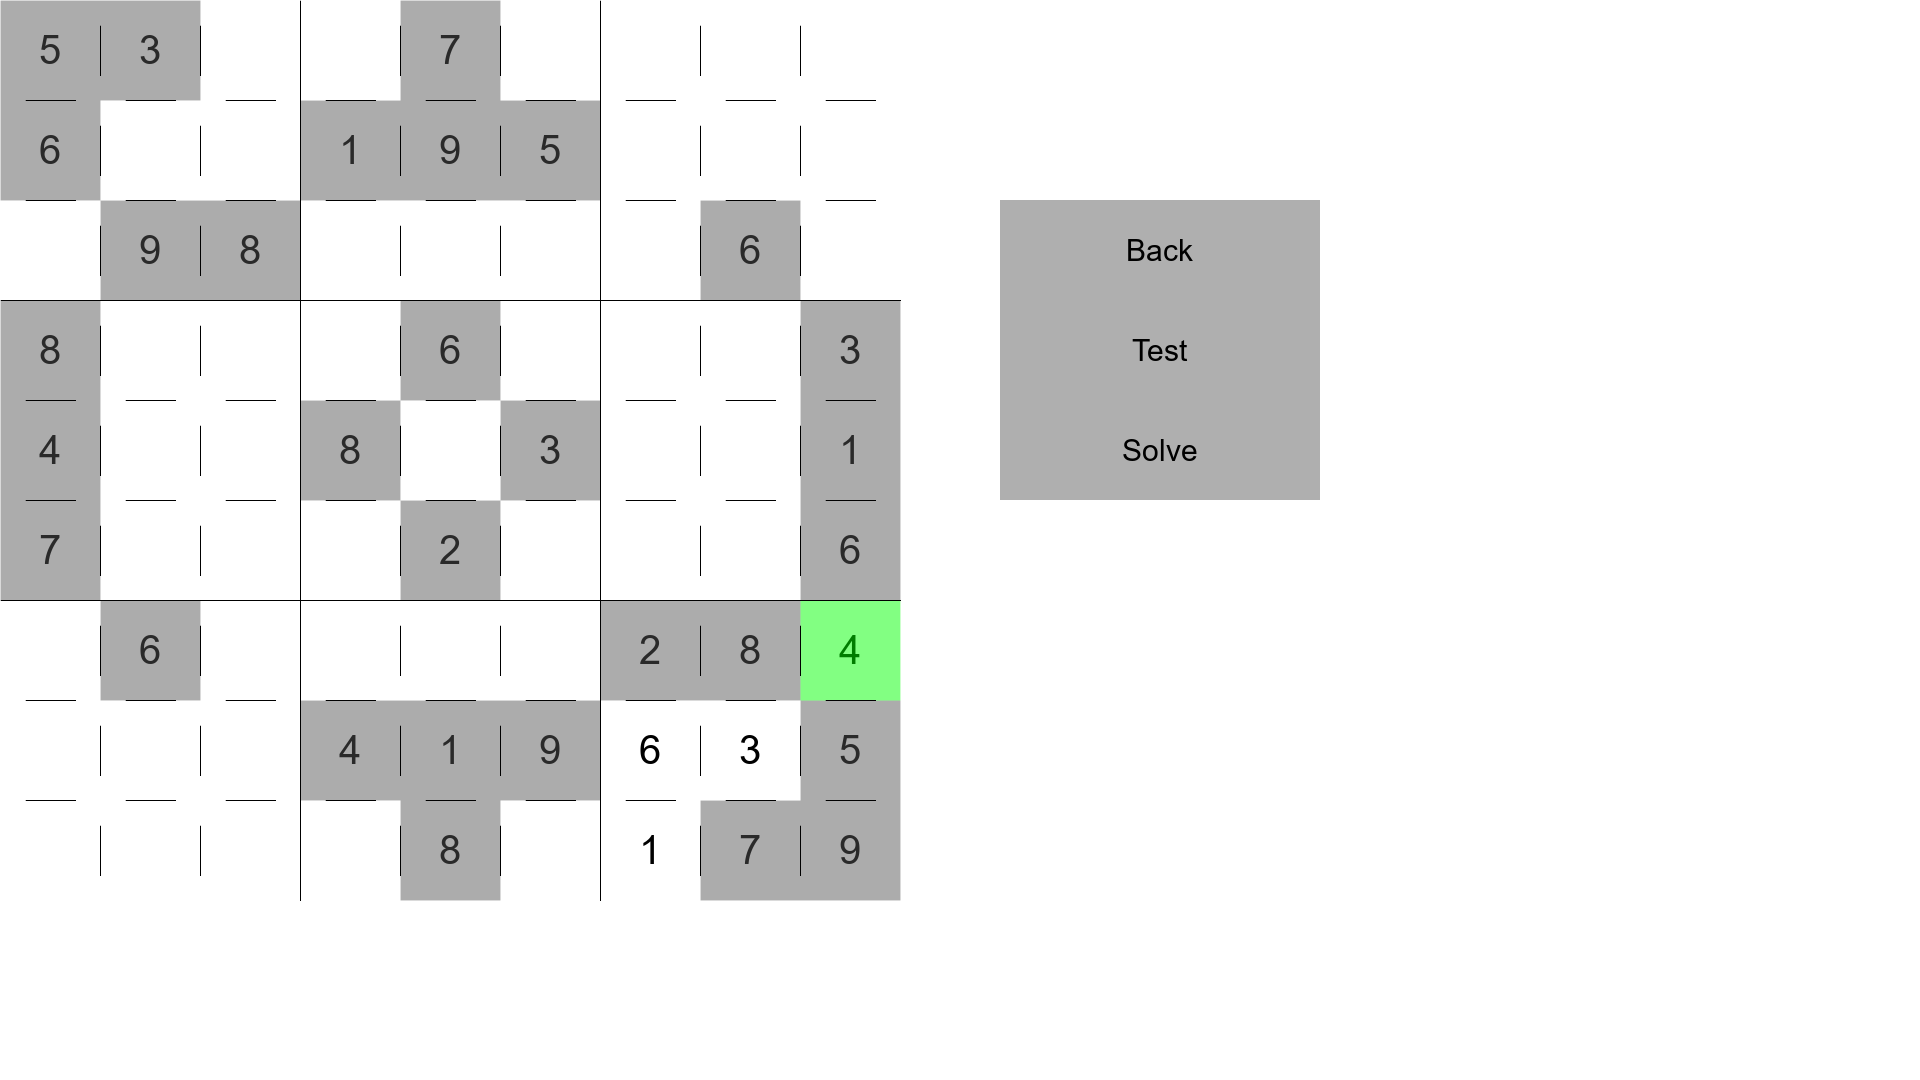
\includegraphics[width=14cm]{user} 
	}
	\caption{\label{fig:user} User Input.}
\end{figure}

\begin{figure}[h]
	\centering
	\fboxsep 2mm
	\framebox{
		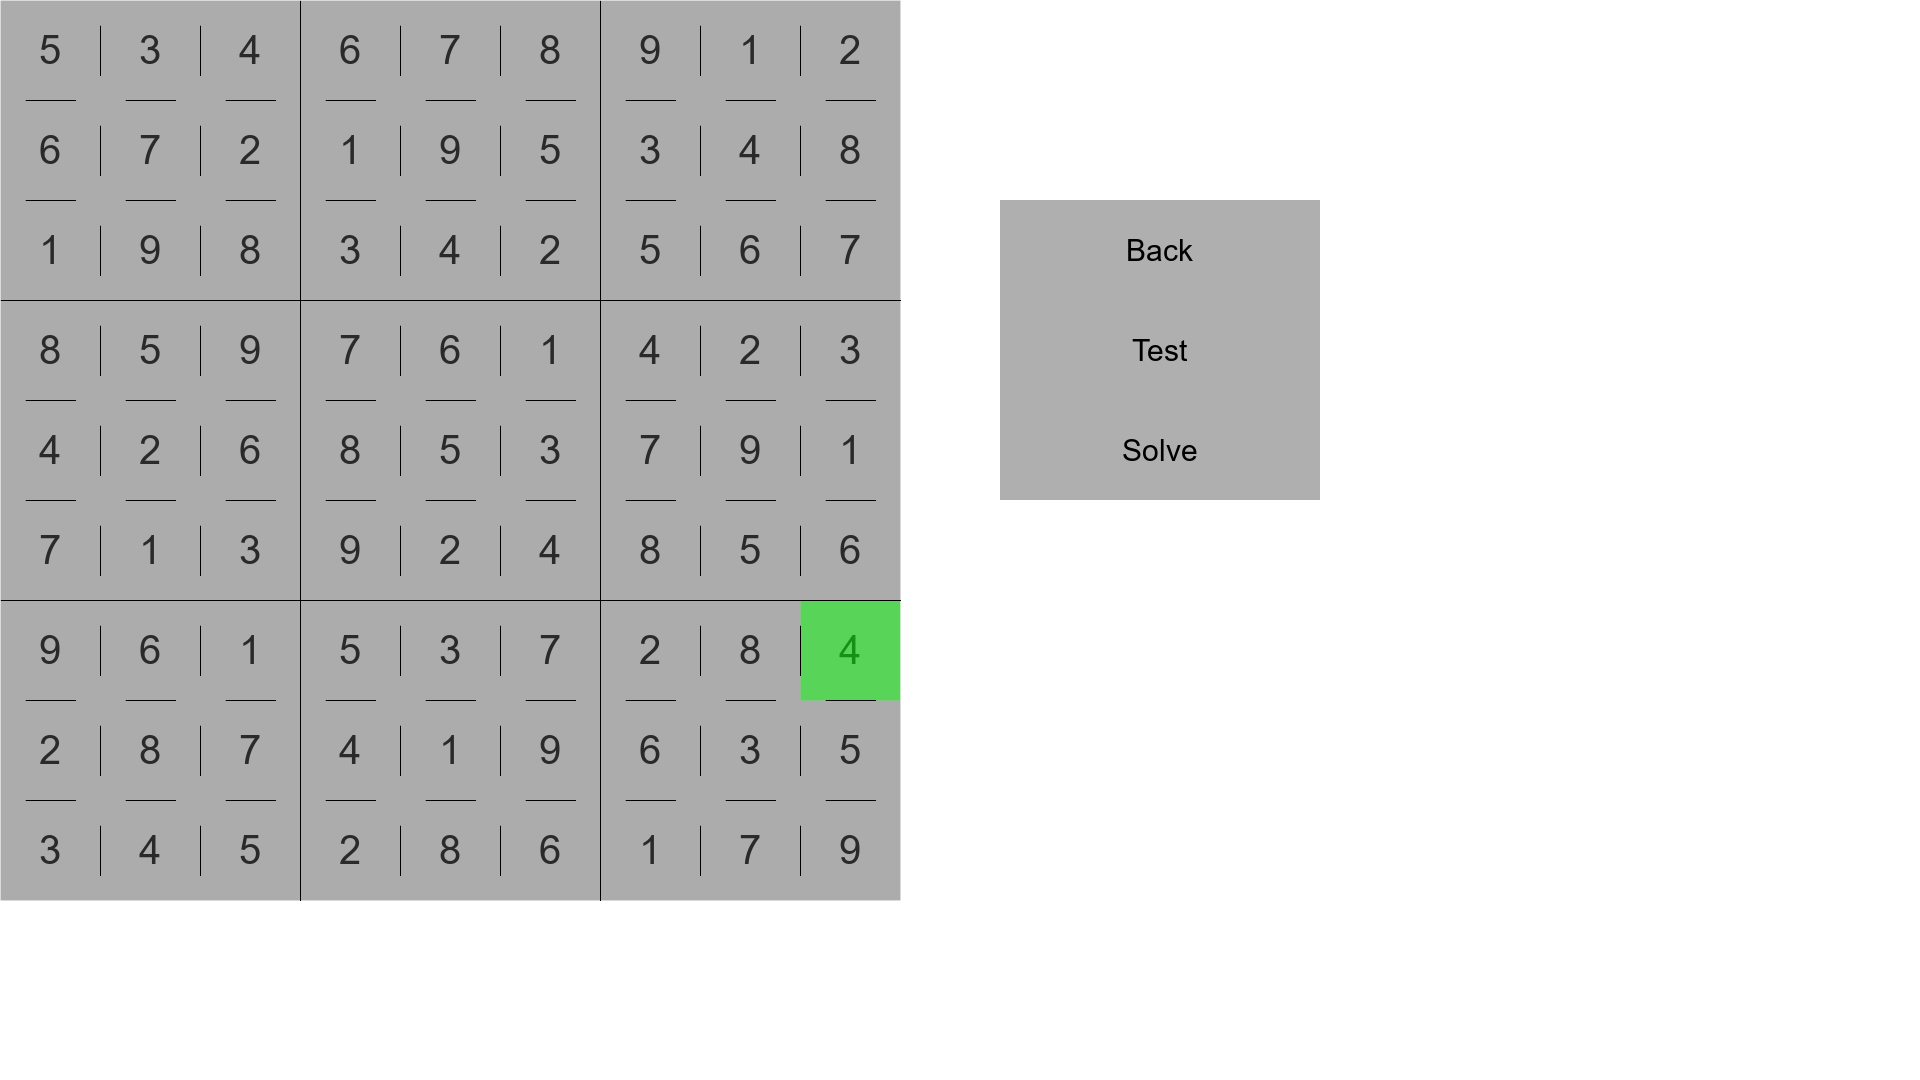
\includegraphics[width=14cm]{solver} 
	}
	\caption{\label{fig:solver} Solver.}
\end{figure}

\newpage

\section*{Complexity and NP Hardness}
\addcontentsline{toc}{section}{Complexity and NP Hardness}

An n\textsuperscript{2} x n\textsuperscript{2} Sudoku is NP complete. Firstly as the problem is in NP, i.e. it can be represented as a decision problem, there either being a solution that can be verified in polynomial time or no solution. Secondly because it is NP hard, as Sudoku can be represented as a graph colouring problem which is known to be NP hard as there is a polynomial time many-one reduction of this to Sudoku which implies it is NP hard.

Verifying a solution takes O(M) or linear time, for an input of grid size M = n\textsuperscript{2} x n\textsuperscript{2}, as each square in the grid only needs to be checked once to see if its value invalidates any constraints on the rows, columns or boxes.

The problem size is largely related to the entire domain and the constraints have negligible effect ~\cite{TSANG:1993}.

\chapter*{Software Engineering}
\addcontentsline{toc}{chapter}{Software Engineering}

In development of my program I used the Agile development cycle to quickly produce an initial working main menu GUI and then continued iterating on this, to extend the application to solve the eight queens problem, then displaying the grid for sudoku and allowing user input and finally solving sudoku as well.

To help me develop my program I am using the Code Blocks IDE, as it comes with many tools and plugins that are useful for developing my program in C++, this made it significantly easier to set up SDL as well as produce documentation for my code.

For unit testing I used the catch2 library, as this was the simplest to set up.

I am using the Google programming standards from their C++ guide, as well as a plugin to automatically format my code and all warning flags for the compiler.

For tasks I am using githubs project boards to keep track of bugs and new features to be added.

I have also been doing system testing on my release candidate branches, as well as testing the application on other machines.

I have used several design patterns to improve the code, such as the flyweight design pattern to limit the number of objects created for numbers.

\chapter*{Professional Issues}
\addcontentsline{toc}{chapter}{Professional Issues}

When developing my program I used C++ with SDL, this meant I had to deal with the SDL library being written in C, which caused issues when trying to write my code to a C++ standard of software engineering and meant I had to use for example raw pointers instead of references because the libraries methods had these as arguments. The library also made frequent use of C structs where C++ classes would have been better making use of smart pointers difficult as I had to specifically call destructor methods for e.g. SDL textures.

This is important as library compatibility can stop developers making full use of the language and can stop the program from being as portable, it also means that it is more difficult to follow strict software engineering principles, although I could implement the interface design pattern to better use the libraries functionality, and keep the code maintainable.

\chapter*{Conclusion and self evaluation}
\addcontentsline{toc}{chapter}{Conclusion and self evaluation}

In conclusion, this project achieved most of the aims and objectives set out at the beginning in the plan, I have created a working professional program with a very functional GUI and have implemented the solving and generating algorithms, as well as saving, loading and benchmarking. The programs code in C++ and SDL has amounted to many thousands of lines of code, but is still very readable and maintainable and fulfils the software engineering principles and processes that I set out to use when developing the program. I have also been able to cover many aspects of theory relating to constraint satisfaction problems and algorithms relating to this, as well as optimizations for them while researching this project. I have also made many uses of design patterns to refactor my programs code, such as the GUI rewrite I did to implement the state design pattern, which ended up requiring changes to many classes, as well as additional ones and made the code much simpler to read and maintain, while also improving my understanding of design patterns and C++ abstract classes and inheritance.

To improve my program further I was planning on extending it so that the user could change the difficulty settings so that they can decide how difficult a sudoku to generate and if they want to generate a larger grid, which I had tested already with hardcoded changes, this would have also required changes to the input process used for placing numbers in squares so that a buffer was used to keep track of what the user has inputted as a number so far, so that numbers above 9 could be entered without dedicated keys for them, I could then reset this buffer when the user clicks off the square. I also intended on allowing the user to make constraints notes for a square using ctrl and numbers, as well as making navigating the grid easier with arrow hotkeys to move from square to square. I would have also liked to finish implementing more solving algorithms and optimizations to better solve the constraint satisfaction problem, but I spent too long designing an efficient implementation of this in pseudocode and didn't want to implement it in the program so close to the deadline as it might have broken something.

I also struggled in getting the testing library I planned on using set up and working, and as such I was not able to add tests for many of my programs methods. I would have liked to have dedicated some time to doing some proper background research to learn how the library worked and how to set it up in my IDE and use it, but ended up using this time to work on the program instead. This is one of the issues of using C++ for my project as I already had previous experience and knowledge of using junit in testing java code, which would have made this process easier, but would have not allowed me to learn as many new things from my project, having started this with only a basic understanding of C and never having done a large project in it.

However I was able to develop a large program with thousands of lines of code over tens of classes, with good software engineering principles and a professional looking GUI and an algorithm that could generate many unique different and difficult sudokus for the user of the program to attempt to solve.

This project also helped me learn skills relevant to developing large programs, including the use of a repository and making modular code that is easy to read and maintain.

\newpage
\begin{thebibliography}{99}
	\addcontentsline{toc}{chapter}{Bibliography}
	\bibitem{TSANG:1993} Edward Tsang (1993). \emph{Foundations of Constraint Satisfaction}.
	\newline
	As Sudoku can be described as a Constraint Satisfaction problem, it is relevant to research what these are and how to solve them, this book has detailed explanations and examples that will help in solving the Eight Queens problem and using CSP algorithms.
	\bibitem{RUSSELL:2016} Stuart Russell and Peter Norvig (2016). \emph{Artificial Intelligence: A Modern Approach -- Third Edition}.
	\newline
	This book has relevant information and examples of AI algorithms like backtracking search and efficient algorithms like alpha/beta pruning that will be helpful in generating and solving Sudoku puzzles.
	\bibitem{MITCHELL:2013} Shaun Mitchell (2013). \emph{SDL Game Development}.
	\newline
	As the GUI will be made using SDL 2.0, it is relevant to use this book to see examples of GUI initialisation code and documentation on the framework, which will be helpful in creation the screens to display and solve the Sudoku puzzles.
	\bibitem{GAMMA:1995} Erich Gamma, Richard Helm, Ralph Johnson and John Vlissides (1995). \emph{Design Patterns: Elements of Reusable Object-Oriented Software}.
	\newline
	This books provides a detailed overview of all Design Patterns, which will be relevant when writing about the Software Engineering Processes used in the program and will be helpful in providing examples of how to refactor program code to include Design Patterns.
	\bibitem{NORVIG:2019} Peter Norvig. \emph{norvig.com/sudoku.html}.
	\newline
	This website provides useful examples of the backtracking algorithms and how they should work to solve a Sudoku puzzle of any difficulty.
	\bibitem{WIKIPEDIA:2019} Wikipedia. \emph{en.wikipedia.org/wiki/Sudoku\_solving\_algorithms}.
	\newline
	This website provides a good overview of different ways of solving a Sudoku puzzle, which could be used to find other more efficient algorithms to use, such as modelling the Sudoku puzzle as an exact cover problem and finding the solution with the dancing links algorithm.
	\bibitem{KRISTANIX:2019}  Kristanix. \emph{kristanix.com/sudokuepic/sudoku-solving-techniques.php}.
\end{thebibliography}

\chapter*{Project Diary}
\addcontentsline{toc}{chapter}{Project Diary}

The following is a summary of the project diary notes I have made during the development of the project program, as I have not had time to type them up until now. I started development of the program by setting up the repository, this included setting up the SDL libraries in Code Blocks, I had some trouble getting my program to compile at first and spent some time modifying the compiler flags, once this was done I then tested the libraries had been initialised properly by running the program with some example SDL rendering code.

Next using the book SDL Game Development for examples, I set up the main game loop to run the program, then I created a class for the buttons on the main menu, this involved handling events when the user clicks on them, as well as rendering them on the screen, I then added these buttons into the game loop and found a bug where a user could click through buttons, i.e. if a button navigated to another screen, then another button in the same place as the button previously clicked would also be clicked, I did not notice this at first, but later it caused me to think another part of the program was broken, after investigating I fixed this by only handling events on the screen before any navigation, rather than updating the current screen immediately, this way I was not changing a condition for the loop while it was running.

During testing of the program I noticed that the CPU usage was very high, this was clearly because the program was rendering new frames as fast as possible, I decided to limit the frame rate to 60 as this is a common refresh rate for monitors and did not use the CPU nearly as much, but realistically this could be much lower as there are no animations or advanced graphics being displayed.

After this I decided to work on displaying the grid for Sudoku, to start I had to allow navigation between screens and update the rendered buttons as well as handling the events for this screen, I rendered lines to separate the squares and then rendered the values of these squares, when testing that this displayed correctly, the program quickly crashed, as well as my computer, as this did not involve any input from me, it was obviously a memory leak, I confirmed this and found that the number objects texture representations were being created every frame without the last frames texture being destroyed, to fix this I first destroyed the texture before creating a new one, then decided it would clearly be more efficient to just store this texture in the object instead of wasting time creating and destroying textures every frame.

While testing the program and the displaying of the grid, I noticed that the numbers that were being rendered were blurred, I found out that this was because SDL was stretching the number texture to fill the square on the grid, to fix this I just had to render the texture in the centre of the square.

I then handled user events so that the user could select a square by clicking, and then modify it using the number keys.

To improve the User Experience, I changed the GUI so that lines within a box were dotted, as well as implementing overlays to show a selected square as well as locked squares, I also fixed the storing of textures to be rendered, this had previously not been working correctly and was drawing empty squares on the screen for example, I then realised it was because I was using the position on the screen when rendering to the texture that would be stored, but the texture was only exactly the size of what needed to be rendered on it, meaning it would in most cases render outside the texture, I fixed this by creating another position rectangle to render it correctly.

To start on the implementation of the solver for Sudoku, I first needed to be able to check the constraints, so I implemented a method to do this, which counted all the instances of a number in a row, column or box and if there was more than one there would be a conflict, I then tested this on the Sudoku grid using the GUI and modifying squares values to make sure it worked as expected.

Next I implemented the method that would actually solve the Sudoku puzzle, it worked by using a recursive backtracking search, going through all squares on the grid that were not locked, then trying all the numbers from one to nine and checking if there were any conflicts, if there were not it would then move onto the next square, otherwise it would try the next number, once it had tried all numbers it would backtrack as clearly a previous number was not correctly placed. I originally considered copying the grid every time the solver moved onto the next square as a standard recursive algorithm would do, however this clearly would be a costly process in both time and space, considering that the grid contained many entry objects, therefore I decided to partially implement a backtracking search by modifying the grid directly as the solver searched through the grid for the solution.

I then used similar methods and algorithms to solve the Eight Queens problem, adapting the methods as necessary, I considered using inheritance for this as the grid class is similar, but decided against this at the time as the puzzles are sufficiently different, although they have similar GUI displays.

I also added a continue button to the main menu to allow the user to return to the Sudoku puzzle they were previously attempting to solve if they had returned to the main menu, I also improved my code by using list initialisation in constructors as this was previously inefficient and not effective C++, as the compiler was warning me about.

To finish my program ready for the Interim Review, I also implemented some more Design Patterns, this involved making several classes Singletons, as well as implementing the Flyweight Design Pattern for number objects, to reduce the amount of memory be used unnecessarily.

\label{endpage}



\end{document}

%\end{article}
